\section{Aufbau}\label{sec:aufbau}
Wie in \autoref{fig:aufbau} zu sehen, besteht der Versuchsaufbau aus einem Laserrohr, welches mit dem aktiven Medium, einem \ce{He}-\ce{Ne}-Gasgemisch gefüllt ist, dem Resonator in Form von zwei Spiegeln und einem Justierlaser mit der Wellenlänge $\lambda=\SI{523}{\nano\meter}$ inklusive Blende zur Justage des Hauptlasers. Alle Komponenten sind mithilfe von Reitern auf einer Schiene platziert, um kontrollierte Abstandskonfigurationen zu ermöglichen.

\begin{figure}[H]
    \centering
    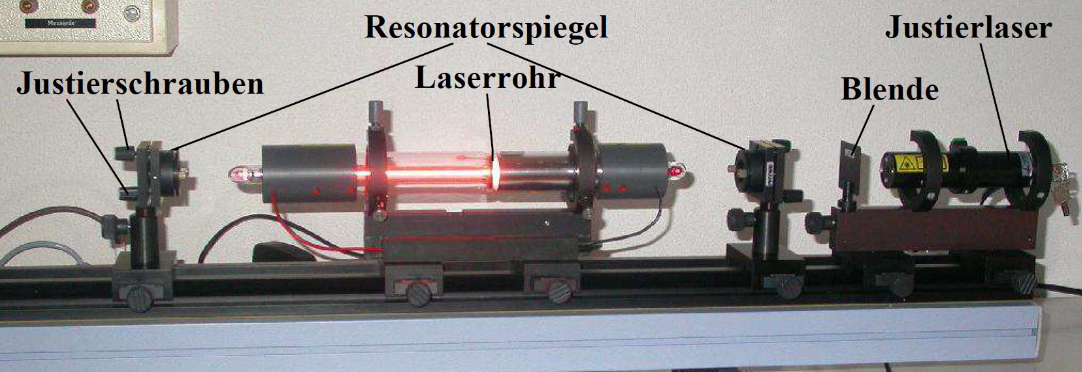
\includegraphics[scale=0.5]{Ressourcen/aufbau.png}
    \caption{Komponenten und Komposition des Verwendeten \ce{He}-\ce{Ne}-Lasers\cite{anleitung}}\label{fig:aufbau}
\end{figure}

\subsection{Laserrohr und Resonator}
Im Laserrohr der Länge $l=\SI{408}{\centi\meter}$ und des Durchmessers $d = \SI{1.1}{\milli\meter}$ bilden Elektroden die Energiepumpe, um für eine Inversion des Gasgemischs zu sorgen und die Enden sind mit Brewsterfenstern zur Selektion einer Polarisationsrichtung versehen. Am Laserrohr sowie den Resonatorspiegeln befinden sich Justierschrauben, welche die Ausrichtung und somit die stabile Funktion des Lasers ermöglichen.

\subsection{Spiegel}
Die zur Verfügung stehenden Spiegel können \autoref{tab:spiegel} entnommen werden.

\begin{table}[H]
  \centering
  \caption{Mögliche Spiegel im Versuchsaufbau und Eigenschaften dieser\cite{anleitung}}
  \begin{tabular}{c | c | c}
    \toprule
    Spiegel & Bezeichnung & Oberflächenbeschaffenheit \\
    \midrule
    plan    & flat/flat            & HR (high reflectivity) R $\geq 99\%$ \\
    konkav  & r=1000 mm/flat       & HR (high reflectivity) R $\geq 99\%$ \\
    konkav  & r=1400 mm/flat       & HR (high reflectivity) R $\geq 99\%$ \\
    konkav  & r=1400 mm/flat       & OC (out coupling) T=1.5,\dots 1.8\% \\
    \bottomrule
  \end{tabular}
  \label{tab:spiegel}
\end{table}

\subsection{Messkomponenten}
Zusätzlich werden verschiedene Komponenten wie Photodioden, Gitter, Mikrometerschrauben und Polarisatoren zur Erfassung verschiedener Strahlungseigenschaften verwendet.
